\section{Modellierung der Dynamik}

\noindent
In der \textbf{statischen Modellierung} im Domänenmodell werden Klassen in ihrem \textit{Zusammenhang} modelliert.\\

\noindent
Das statische Modell gibt keine Informationen über den Zustand eines Objektes oder wie Botschaften untereinander ausgetauscht werden, und wie sich Objekte / Klassen daraufhin verhalten.\\

\noindent
Um darzustellen, wie sich Klassen oder Objekte verhalten, nutzt man das \textbf{dynamische Modell}.\\

\noindent
Hierzu werden in der \textbf{Analyse} Zustände und Zustandsübergänge eines Systems sowie Aktivitäten modelliert.\\
Grundlage sind Dokumente der Anforderungen, die \textbf{Verhalten} beschreiben, also\textbf{User Stories}, \textbf{Anwendungsfälle} und \textbf{Szenarien}.\\
Die dort beschriebenen Abläufe werden bei der dynamischen Modellierung konkretisiert und genauer definiert.

\subsection*{Zustände und Zustandsänderungen}
\textbf{Systeme} (\textit{Klassen}, \textit{Subsysteme}, \textit{Anwendungen}) können \textbf{Zustände} besitzen, die sich verändern können.\\

\noindent
Oft sind nur Übergänge zwischen bestimmten Zuständen möglich.\\

\noindent
Die grafische Darstellung dieses Verhaltens erreicht man über \textbf{UML-Zustandsdiagramme} (s. Abbildung~\ref{fig:statediagram}).

\begin{figure}
    \centering
    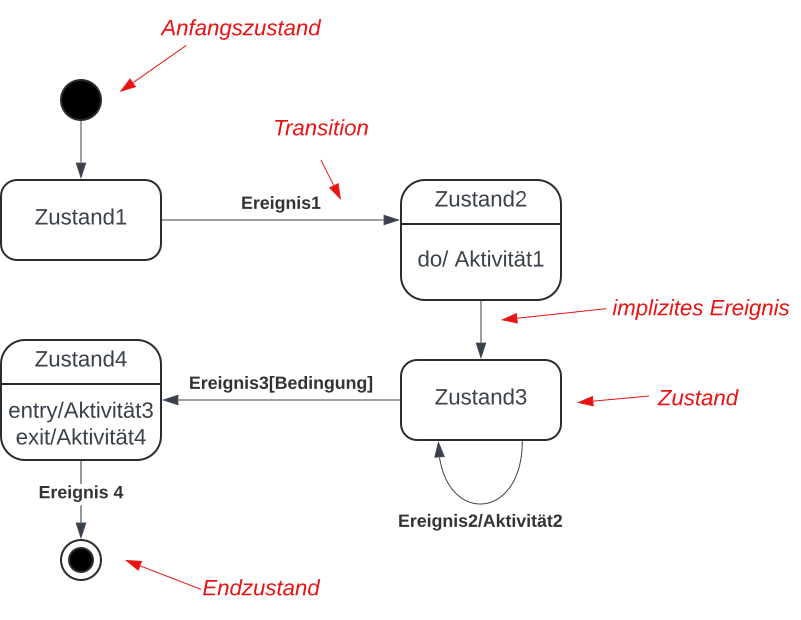
\includegraphics[scale=0.4]{part two/Objektorientierte Analyse/img/statediagram}
    \caption{In der Objektorientierung werden Zustandsautomaten mit Hilfe von Zustandsdiagrammen (\textit{statechart diagram}) dargestellt. Die in der Abbildung gezeigten /do/entry/exit-Aktivitäten werden innerhalb eines Zustands aufgerufen. Ein \textit{implizites Ereignis} (auch: \textit{Beendigungsereignis}) liegt vor, wenn die mit dem Vorgängerzustand verbundene Verarbeitung beendet ist, und eine \textit{Transition} in den Folgezustand führt. (Quelle: in Anlehnung an~\cite[90, Abb. 2.11-6]{Bal05})}
    \label{fig:statediagram}
\end{figure}

\subsection*{Aktivitätsdiagramme}
Bei Zustandsdiagrammen erschließt sich der Ablauf von Aktivitäten meist nur indirekt, da bspw. keine Auskunft über die beteiligten Akteure modelliert werden können.\\

\noindent
Aus diesem Grund verwendet man \textbf{UML-Aktivitätsdiagramm}\footnote{
s. ``15 Activities``, S. 373, \url{https://www.omg.org/spec/UML/2.5.1/PDF}, abgerufen 22.04.2024
}, in denen Aktivitäten in ihrer möglichen Abfolge und ihrer Zuordnung zu Akteuren modelliert werden (s. Abbildung~\ref{fig:activitydiagram}).\\

\begin{figure}
    \centering
    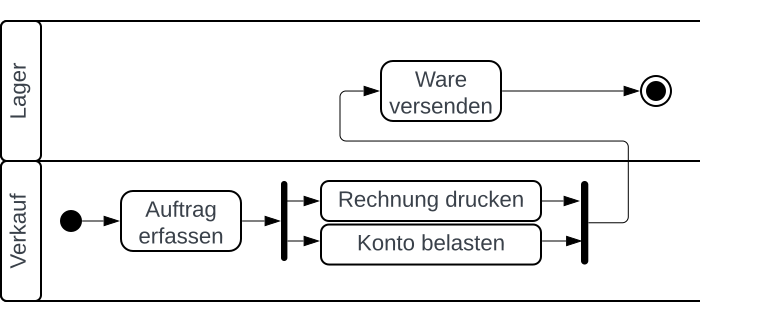
\includegraphics[scale=0.5]{part two/Objektorientierte Analyse/img/activitydiagram}
    \caption{Beispiel für ein Aktivitätsdiagram (\textit{activity diagram}). (Quelle: in Anlehnung an~\cite[77, Abb. 2.9-14]{Bal05})}
    \label{fig:activitydiagram}
\end{figure}

\noindent
Darüberhinaus kann mit Aktivitätsdiagrammen  auch der Fluss von Informationen und die Auswirkung auf Objekte dargestellt werden.\\

\vspace{2mm}
\begin{tcolorbox}
Aktivitätsdiagramme sind zur Modellierung von User Stories, Szenarien oder Anwendungsfällen geeignet.
\end{tcolorbox}
\vspace{2mm}